\documentclass[12pt,]{article}
\usepackage{lmodern}
\usepackage{amssymb,amsmath}
\usepackage{ifxetex,ifluatex}
\usepackage{fixltx2e} % provides \textsubscript
\ifnum 0\ifxetex 1\fi\ifluatex 1\fi=0 % if pdftex
  \usepackage[T1]{fontenc}
  \usepackage[utf8]{inputenc}
\else % if luatex or xelatex
  \ifxetex
    \usepackage{mathspec}
  \else
    \usepackage{fontspec}
  \fi
  \defaultfontfeatures{Ligatures=TeX,Scale=MatchLowercase}
\fi
% use upquote if available, for straight quotes in verbatim environments
\IfFileExists{upquote.sty}{\usepackage{upquote}}{}
% use microtype if available
\IfFileExists{microtype.sty}{%
\usepackage[]{microtype}
\UseMicrotypeSet[protrusion]{basicmath} % disable protrusion for tt fonts
}{}
\PassOptionsToPackage{hyphens}{url} % url is loaded by hyperref
\usepackage[unicode=true]{hyperref}
\hypersetup{
            pdftitle={Chapter 2 Draft},
            pdfborder={0 0 0},
            breaklinks=true}
\urlstyle{same}  % don't use monospace font for urls
\usepackage[margin=1in]{geometry}
\usepackage{graphicx,grffile}
\makeatletter
\def\maxwidth{\ifdim\Gin@nat@width>\linewidth\linewidth\else\Gin@nat@width\fi}
\def\maxheight{\ifdim\Gin@nat@height>\textheight\textheight\else\Gin@nat@height\fi}
\makeatother
% Scale images if necessary, so that they will not overflow the page
% margins by default, and it is still possible to overwrite the defaults
% using explicit options in \includegraphics[width, height, ...]{}
\setkeys{Gin}{width=\maxwidth,height=\maxheight,keepaspectratio}
\IfFileExists{parskip.sty}{%
\usepackage{parskip}
}{% else
\setlength{\parindent}{0pt}
\setlength{\parskip}{6pt plus 2pt minus 1pt}
}
\setlength{\emergencystretch}{3em}  % prevent overfull lines
\providecommand{\tightlist}{%
  \setlength{\itemsep}{0pt}\setlength{\parskip}{0pt}}
\setcounter{secnumdepth}{0}
% Redefines (sub)paragraphs to behave more like sections
\ifx\paragraph\undefined\else
\let\oldparagraph\paragraph
\renewcommand{\paragraph}[1]{\oldparagraph{#1}\mbox{}}
\fi
\ifx\subparagraph\undefined\else
\let\oldsubparagraph\subparagraph
\renewcommand{\subparagraph}[1]{\oldsubparagraph{#1}\mbox{}}
\fi

% set default figure placement to htbp
\makeatletter
\def\fps@figure{htbp}
\makeatother

\usepackage{setspace}\doublespacing
\usepackage{booktabs}
\usepackage{longtable}
\usepackage{array}
\usepackage{multirow}
\usepackage{wrapfig}
\usepackage{float}
\usepackage{colortbl}
\usepackage{pdflscape}
\usepackage{tabu}
\usepackage{threeparttable}
\usepackage{threeparttablex}
\usepackage[normalem]{ulem}
\usepackage{makecell}
\usepackage{xcolor}

\title{Chapter 2 Draft}
\author{}
\date{\vspace{-2.5em}}

\begin{document}
\maketitle

Here I'm going to try to understand our data a bit better and state our
hypothesis.

First I start with an abstract that could be our guide for hypothesis
testing and analyses.

\section{Abstract (draft)}\label{abstract-draft}

Plant pollinator interactions are a keystone process for ecosystem
functioning. However, we lack comprehensive information from both plants
and pollinators that can inform from this mutualistic interaction
worldwide. In order to tackle this, we have selected 30 networks
distributed across the world and looked for key floral traits of
plant-pollinator interactions for a total of 1600 species. Here we look
how these floral traits shape the different plant-pollinator networks
and the main fuctional groups of insect pollinating species. Giving the
different nature of the data collated we do not compare across networks
and we focus on the main general patterns/results within network. We
have conducted our analysis at 3 levels, 1) unique networks, 2) metawebs
and by 3) grouping both. We find that specific traits are associated
with different guilds of floral visitors within these networks. We also
highlight the lack of information about traits and the reproductive
biology of the plant species of these networks. Our work shows the
importance of deepen in species traits in order to understand key
processes that can be seen with network metrics and highlights the
importance of elemental ecology for species conservation.

\emph{What sort of data do we have?}

There are approximately 1600 species from 30 different networks. All of
these networks are phytocentric (built from plants). The different
plant-pollinator communities have been studied with very different
sampling effort and methodologies. Therefore, our aim is not to compare
across studies but to create a general picture of how floral traits
shape the different pollinator taxa and network metrics. Here, we
combine the studies with multiple years of sampling and multiple sites
within an area in metawebs. These networks give a broader perspective of
the sampling area and inform about the regional species pool (Noreika et
al. 2019). The data of these networks is quantitative (visitation) or
qualitative (binary), there are in total 19 and 11 networks/metawebs of
each, respectively.

\blandscape

\begin{tabular}{r|l|r|l|l|l|l|l|r|r|r|l|l|l}
\hline
X & BIBTEXKEY & Id\_number & longitude & latitude & country & experiment\_year & unique\_networks & plant\_species & pollinator\_species & network\_size & Sampling\_method & Sampling\_zoo\_phytocentric & Data\_type\\
\hline
1 & 1\_metaweb\_carpobrotus\_Bartomeus\_2008 & 1 & 3.296797 & 42.315336 & Spain & 2005 & 3 & 18 & 37 & 666 & Plots 50*50m with 2 transects (N=3) & Phytocentric & Quantitative\\
\hline
2 & 10\_metaweb\_fang\_huang\_2012 & 10 & 99.63806 & 27.90139 & China & 2008-2010 & 3 & 130 & 247 & 32110 & plots with stratified distribution to include rare plants within 800*250m plot & Phytocentric & Quantitative\\
\hline
3 & 11\_metaweb\_inouye\_1990 & 11 & 135.866667 & 35.166667 & Japan & 1984-1987 & 4 & 114 & 883 & 100662 & Transect from stream and a bog & Phytocentric & Quantitative\\
\hline
4 & 12\_inouye\_1988 & 12 & 148.266667 & -36.45 & Australia & 1983-1984 & 1 & 40 & 85 & 3400 & 26 plots with stratified sampling of 10 minutes in each site & Phytocentric & Quantitative\\
\hline
5 & 13\_metaweb\_kaiser\_bunbury\_2009 & 13 & 57.443254 & -20.452076 & Republic of Mauritius & 2003-2004 & 2 & 96 & 184 & 17664 & 2h per sepecies within a 330*100m plot & Phytocentric & Quantitative\\
\hline
6 & 14\_metaweb\_kaiser\_bunbury\_2014 & 14 & 55.43333 & -4.666667 & Republic of Seychelles & 2007-2008 & 6 & 37 & 341 & 12617 & 2 to 4 transects of 100m, 48 networks in 6 different sites & Phytocentric & Quantitative\\
\hline
7 & 15\_metaweb\_kato\_2000 & 15 & 129.493741 & 28.377248 & Japan & 1996-1999 & 16 & 110 & 609 & 66990 & Transects from a fixed point from forest or meadow with 10 min per site & Phytocentric & Quantitative\\
\hline
8 & 16\_kevan\_1970 & 16 & -71.3 & 81.816667 & Canada & 1967 & 1 & 20 & 91 & 1820 & random walks & Phytocentric & Qualitative\\
\hline
9 & 17\_lundgren\_2005 & 17 & -52 & 71 & Greenland & 2002 & 1 & 17 & 26 & 442 & 20 mins per spp, regular walks within the plot (100*100m), max per spp 4h & Phytocentric & Quantitative\\
\hline
10 & 18\_olesen\_2002\_mauritius & 18 & 57.43 & -20.25 & Republic of Mauritius & 1998-1999 & 1 & 17 & 26 & 442 & 37 quadrats 100*100m & Phytocentric & Quantitative\\
\hline
11 & 19\_mcmullen\_1993 & 19 & -90.600747 & -0.290164 & Ecuador & NA & All islands & 105 & 54 & 5670 & Metaweb from the literature & Phytocentric & Qualitative\\
\hline
12 & 2\_metaweb\_opuntia\_Bartomeus\_2008 & 2 & 3.296797 & 42.315336 & Spain & 2005 & 3 & 13 & 37 & 481 & Plots 50*50m with 2 transects (N=3), Plots 50*50m (N=3) & Phytocentric & Quantitative\\
\hline
13 & 20\_metaweb\_arthurs\_pass\_primack\_1983 & 20 & 171.566667 & -42.95 & New Zealand & 1976-1978 & 1 & 18 & 60 & 1080 & Random census walks & Phytocentric & Qualitative\\
\hline
14 & 21\_metaweb\_cass\_primack\_1983 & 21 & 171.78466 & -43.02823 & New Zealand & 1976-1978 & 1 & 41 & 139 & 5699 & Random census walks & Phytocentric & Qualitative\\
\hline
15 & 22\_metaweb\_craigieburn\_primack\_1983 & 22 & 171.720224 & -43.099531 & New Zealand & 1976-1978 & 1 & 49 & 118 & 5782 & Random census walks & Phytocentric & Qualitative\\
\hline
16 & 23\_ramirez\_1989 & 23 & -61.716667 & 5.583333 & Venezuela & NA & 1 & 48 & 49 & 2352 & Random census walks & Phytocentric & Qualitative\\
\hline
17 & 24\_metaweb\_ramirez\_1992 & 24 & -67.416667 & 8.933333 & Venezuela & 1983,1984,1989 & 1 & 28 & 53 & 1484 & Random census walks, 16 to 20h of sampling per spp & Phytocentric & Qualitative\\
\hline
18 & 25\_metaweb\_robertson\_1929 & 25 & -89.8968771 & 39.278958 & United States & 1997-1899 & NA & 456 & 1044 & 476064 &  & Phytocentric & Qualitative\\
\hline
19 & 26\_small\_1976 & 26 & -75.5 & 45.4 & Canada & 1973 & 1 & 13 & 34 & 442 & 10 hours per spp & Phytocentric & Quantitative\\
\hline
20 & 27\_chaco\_souza\_2018 & 27 & -57.885 & -21.701111 & Brazil & 2008-2009 & 1 & 62 & 89 & 5518 & 37 plots, 15*25m (at least 50m away), spp within the plots depending sampling effort on abundance & Phytocentric & Quantitative\\
\hline
21 & 28\_metaweb\_traveset\_2013 & 28 & -91.012863 & -0.6907 & Ecuador & 2010-2011 & 1 & 60 & 220 & 13200 & Random census walks with a total of 518h & Phytocentric & Quantitative\\
\hline
22 & 29\_metaweb\_bartomeus\_unpublished\_data\_2015 & 29 & -6.16895, -6.304244, -6.280883, -6.371844, -6.43311, -6.428801, -6.555233, -6.555236, -6.506789, -6.761136, -6.660927, -6.667992, -6.680852, -6.752456, -6.675026, -6.222871 & 37.234966, 37.21781, 37.23919, 37.214279, 37.289861, 37.247223, 37.282079, 37.233157, 37.123856, 37.194957, 37.249254, 37.331447, 37.405047, 37.291937, 37.288346, 37.291091 & Spain & 2015 & 16 & 57 & 277 & 15789 & Transects & Phytocentric & Quantitative\\
\hline
23 & 3\_bek\_2006 & 3 & 10.216667 & 56.066667 & Denmark & 2003 & 1 & 37 & 225 & 8325 & Plots 1*1 in 1 ha & Phytocentric & Qualitative\\
\hline
24 & 30\_olesen\_2002\_azores & 30 & -31 & 39.4 & Azores & 2000 & 1 & 10 & 12 & 120 & 33 quadrats 100*100m & Phytocentric & Quantitative\\
\hline
25 & 4\_bundgaard\_2003 & 4 & 10.233333 & 56.066667 & Denmark & 2003 & 1 & 16 & 44 & 704 & Plots 1*1m near the trail & Phytocentric & Qualitative\\
\hline
26 & 5\_metaweb\_chacoff\_2011 & 5 & -68.015892 & -32.008985 & Argentina & 2006-2009 & 4 & 59 & 196 & 11564 & 4plots-1ha & Phytocentric & Quantitative\\
\hline
27 & 6\_metaweb\_dicks\_2002 & 6 & 1.575532; 1.097873 & 52.762395; 52.413173 & England & 2001? & 2 & 23 & 80 & 1840 & 4plots-1ha & Phytocentric & Quantitative\\
\hline
28 & 7\_metaweb\_dupont\_2009 & 7 & 9.1; 9.266667 & 56.1; 56.066667 & Denmark & 2005 & 2 & 31 & 329 & 10199 & 1*1m within 100*500m plot & Phytocentric & Quantitative\\
\hline
29 & 8\_elberling\_1999 & 8 & 18.5 & 68.35 & Sweden & 1994 & 1 & 24 & 118 & 2832 & Transects within plot of 30*50m & Phytocentric & Quantitative\\
\hline
30 & 9\_dupont\_2009\_zackenberg & 9 & -20.5 & 74.5 & Greenland & 1996-1997 & 1 & 31 & 76 & 2356 & Observation by random census walks within 25 ha & Phytocentric & Qualitative\\
\hline
\end{tabular}

\elandscape

\newpage

\textbf{PLOT 1}

Here I show the percentage or orders from the different species without
consider visitation and just richness of species. Therfore, if we have a
network with 4 species from from different orders, each will appear as
25\% within the stack bar of the barplot.

\vspace{4cm}

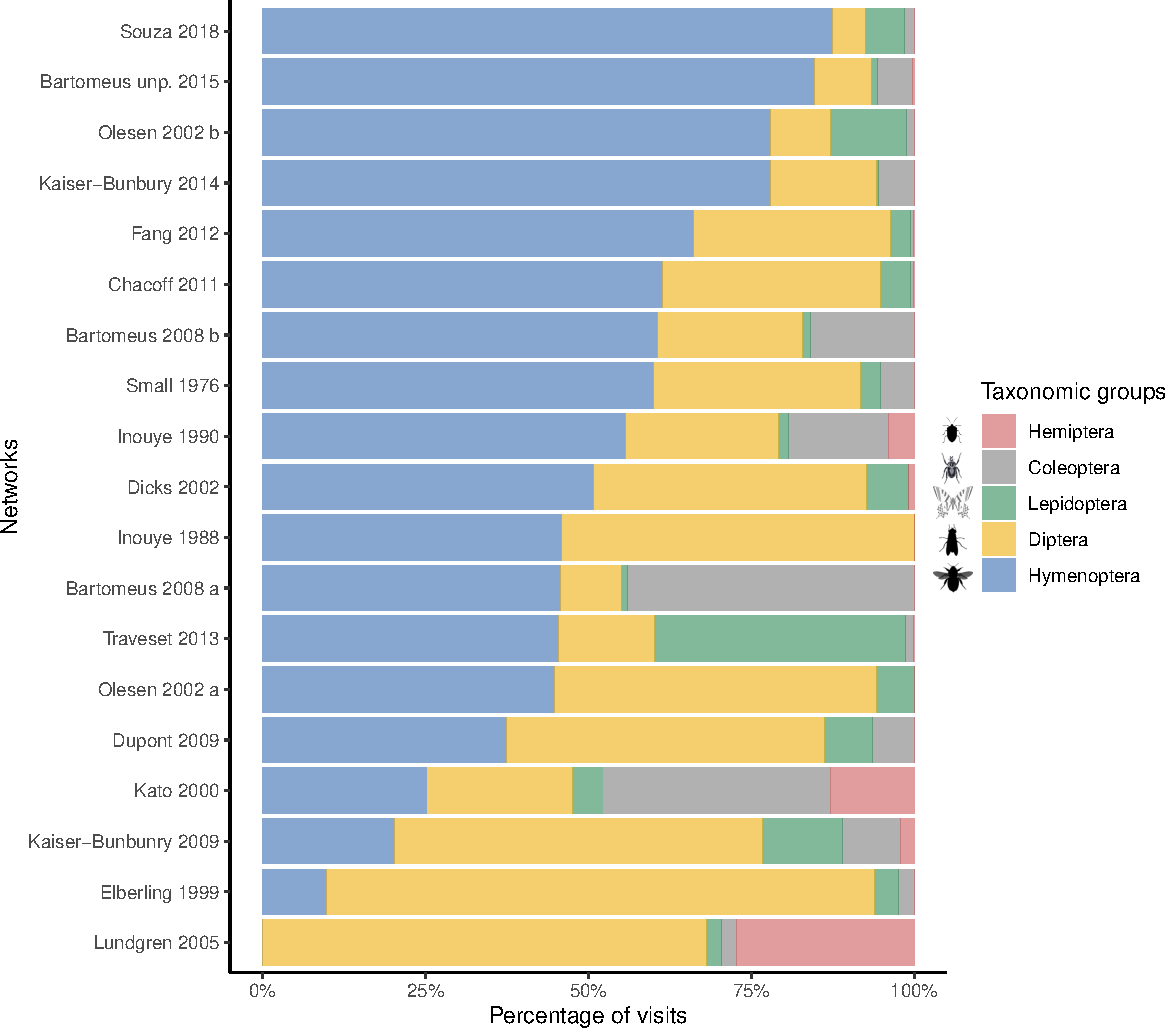
\includegraphics{Draft_files/figure-latex/unnamed-chunk-2-1.pdf}

\newpage

\vspace{4cm}

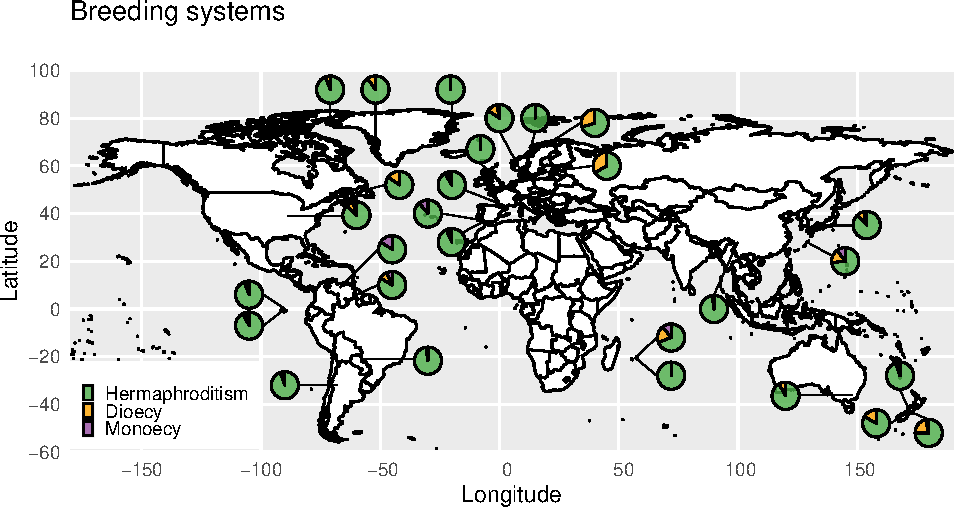
\includegraphics{Draft_files/figure-latex/unnamed-chunk-3-1.pdf}

\newpage
*

*PLOT 2**

\begin{center}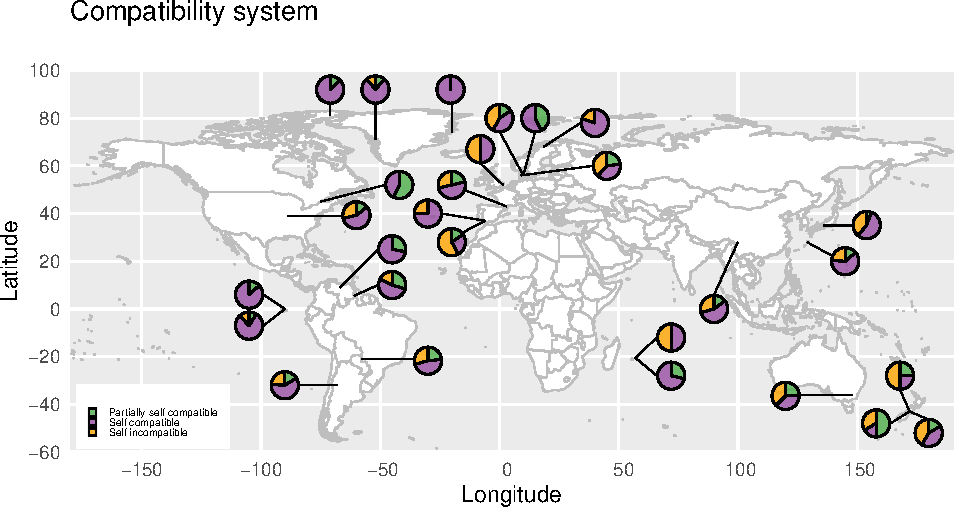
\includegraphics{Draft_files/figure-latex/unnamed-chunk-4-1} \end{center}

\newpage

\textbf{PLOT 3}

\begin{center}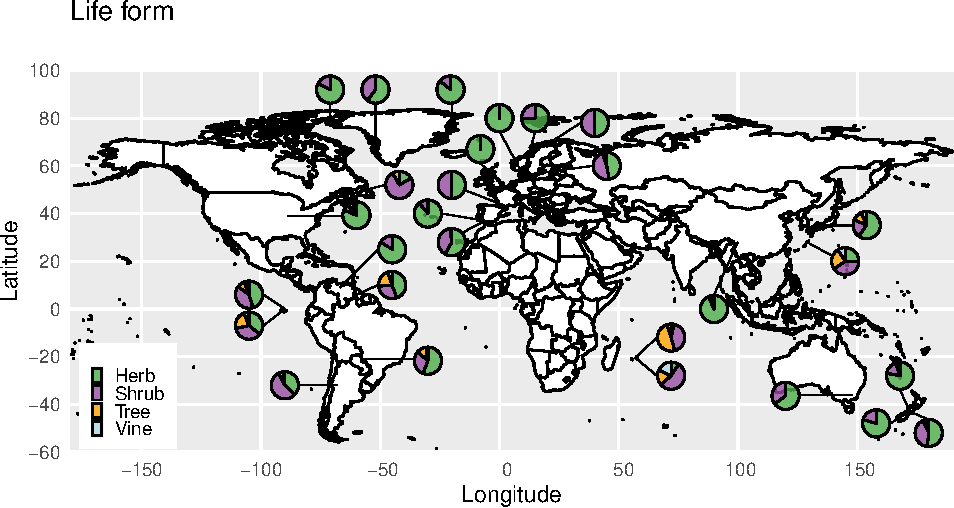
\includegraphics{Draft_files/figure-latex/unnamed-chunk-5-1} \end{center}

\newpage

\textbf{PLOT 4}

\begin{center}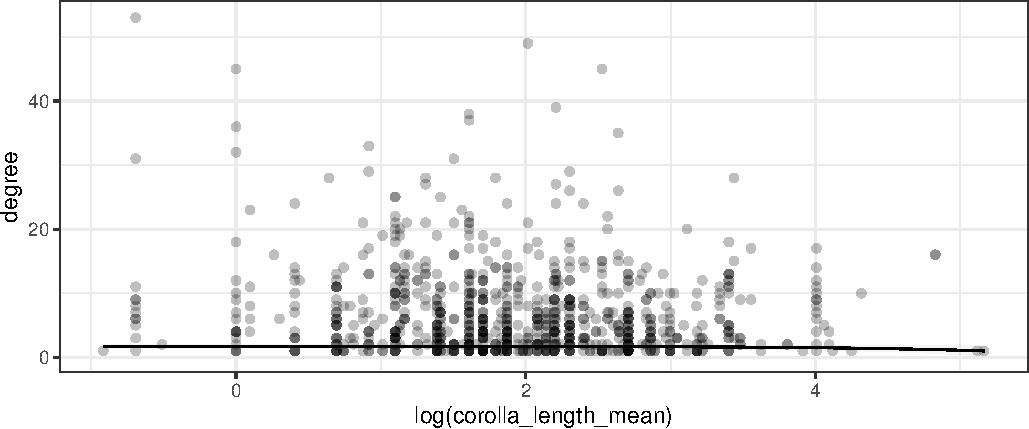
\includegraphics{Draft_files/figure-latex/unnamed-chunk-6-1} \end{center}

\section*{REFERENCES}\label{references}
\addcontentsline{toc}{section}{REFERENCES}

\hypertarget{refs}{}
\hypertarget{ref-noreika2019pollinator}{}
Noreika, Norbertas, Ignasi Bartomeus, Marie Winsa, Riccardo Bommarco,
and Erik Öckinger. 2019. ``Pollinator Foraging Flexibility Mediates
Rapid Plant-Pollinator Network Restoration in Semi-Natural Grasslands.''
\emph{Scientific Reports} 9 (1). Nature Publishing Group: 1--11.

\end{document}
